\documentclass{article}
%\usepackage[margin=1in]{geometry}
\setlength\topmargin{0pt}
\addtolength\topmargin{-\headheight}
\addtolength\topmargin{-\headsep}
\setlength\oddsidemargin{0pt}
\setlength\textwidth{\paperwidth}
\addtolength\textwidth{-2in}
\setlength\textheight{\paperheight}
\addtolength\textheight{-2in}

\usepackage[english]{babel}
\usepackage[utf8]{inputenc}
\usepackage{fancyhdr}
\usepackage{listings}
\usepackage{graphicx}
\usepackage{xcolor}


\definecolor{codegreen}{rgb}{0,0.6,0}
\definecolor{codegray}{rgb}{0.5,0.5,0.5}
\definecolor{codepurple}{rgb}{0.58,0,0.82}
\definecolor{backcolour}{rgb}{0.95,0.95,0.92}


\usepackage{booktabs}
\usepackage{pgfplotstable}



\lstdefinestyle{mystyle}{
	backgroundcolor=\color{backcolour},
	commentstyle=\color{codegreen},
	keywordstyle=\color{magenta},
	numberstyle=\tiny\color{codegray},
	stringstyle=\color{codepurple},
	basicstyle=\ttfamily\footnotesize,
	breakatwhitespace=false,
	breaklines=true,
	captionpos=b,
	keepspaces=true,
	numbers=left,
	numbersep=5pt,
	showspaces=false,
	showstringspaces=false,
	showtabs=false,
	tabsize=2
}
\lstset{style=mystyle}

\title{Machine Learning Project 3 Neural Networks}
\author{Pedram Safaei, Ian Grant }
\date{December 2nd}

\begin{document}

\maketitle

\section{compute\_Z}
\subsection{Explanation}

\begin{lstlisting}[language=Python]
sample code 
\end{lstlisting}


\section{compute\_covariance\_matrix}
\subsection{Explanation}

\begin{lstlisting}[language=Python]
sample code 
\end{lstlisting}

\section{find\_pcs}
\subsection{Explanation}

\begin{lstlisting}[language=Python]
sample code 
\end{lstlisting}

\section{project\_data}
\subsection{Explanation}

\begin{lstlisting}[language=Python]
sample code 
\end{lstlisting}

\section{compress\_images}
\subsection{Explanation}
The \textbf{compress\_images} function takes in a \textbf{DATA} array and an int \textbf{k} the number of principal components to use. It uses PCA to get the principal components to compress the images that were given as input by doting the principal component with Z*. Then using reshape() the image is returned to it's original aspect ratio instead of being flattened. 
\begin{lstlisting}[language=Python]
def compress_images(DATA,k):
    exists = os.path.exists("Output")
    if not exists:
        os.mkdir('Output')
    #for each pic in the data arr
    Z = pca.compute_Z(DATA)
    COV = pca.compute_covariance_matrix(Z)
    L, PCS = pca.find_pcs(COV)
    Zstar = pca.project_data(Z,PCS,L,k,0)
    PCS = PCS[:, :k]
    PCS = PCS.T
    compress = np.dot(Zstar, PCS)
    compress = compress.T
    for j in range(0, len(compress)):
        py.imsave('Output/out%d.png'%j,compress[j].reshape(60,48),vmin=0,vmax=255,cmap='gray',format='png')
\end{lstlisting}

\section{load\_data}
\subsection{Explanation}
The load\_data function takes in a \textbf{inputdir} it loads each image found in the directory into a temp var to then be flattened and loaded into the \textbf{data} var to be returned and used by compress\_images.

\begin{lstlisting}[language=Python]
def load_data(input_dir):
    exists = os.path.exists(input_dir)
    if not exists:
        print("Can't find input dir")
        return 
    dataimg = []
    finalresult = []
    input = input_dir
    for dir, child, datas in os.walk(input):
        for data in np.sort(datas):
            image = py.imread(input+ data, 'pgm')
            image = image.flatten()
            dataimg.append(image)
    finalresult = np.array(dataimg)
    finalresult = finalresult.astype(np.float)
    finalresult = finalresult.transpose()
    return finalresult
\end{lstlisting}

\section{Compressed images from DATA/TRAIN}
\subsection{10}
\subsection{100}
\subsection{500}
\subsection{1000}
\subsection{2000}




% 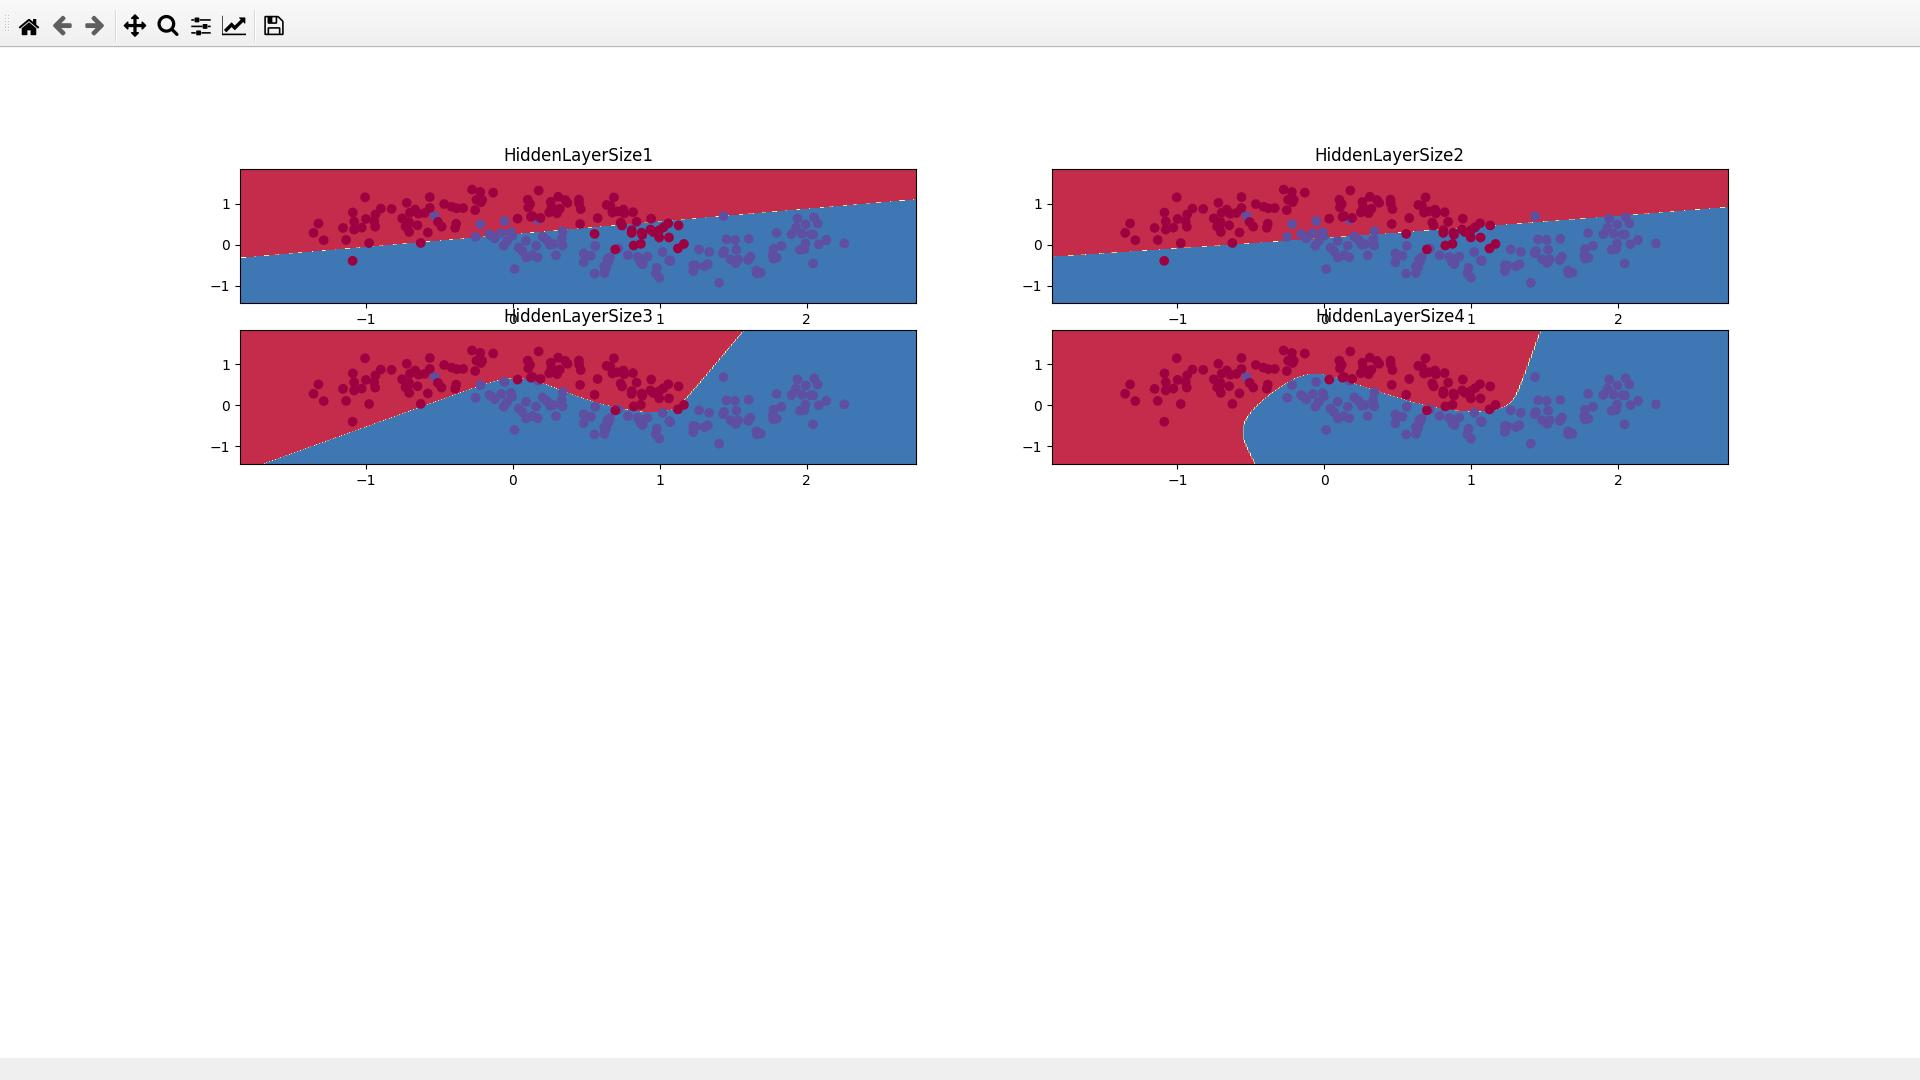
\includegraphics[scale=.25]{plot.jpg}
\end{document}
